\section{Hyperparameters \& Dimensionality}
\begin{frame}{Addressing Overfitting}
    \centering
    \large \textit{Since we cannot trust the training error, we need a systematic approach to validate our models.}
    
    \vspace{0.8cm}
    
    \begin{columns}[T]
        \begin{column}{0.3\textwidth}
            \begin{block}{\centering1. Detect:}
                \centering
                \textbf{Splitting Data}\\
                (Holdout, K-Fold)
            \end{block}
        \end{column}
        \begin{column}{0.3\textwidth}
            \begin{block}{\centering2. Measure:}
                \centering
                \textbf{Metrics}\\
                (Accuracy, MSE, F1, AUC)
            \end{block}
        \end{column}
        \begin{column}{0.3\textwidth}
            \begin{block}{\centering3. Mitigate:}
                \centering
                \textbf{Strategies}\\
                (Regularization, More Data, Better Features)
            \end{block}
        \end{column}
    \end{columns}
    
    \vspace{0.5cm}
    \centering
    \small $\rightarrow$ \textit{Step 1: How to simulate "unseen data" using Splits.} \\
    \small $\rightarrow$ \textit{Step 2: How to measure performance using Metrics.} \\
    \small $\rightarrow$ \textit{Step 3: How to mitigate overfitting.}
\end{frame}

% --- PART 3: REDUCTION (Fixes) ---
% --- PART 3: REDUCTION (MITIGATION) ---
% --- PART 3: REDUCTION (MITIGATION) ---


% --- SLIDE 1: MODEL COMPLEXITY & HYPERPARAMETERS ---
\begin{frame}{Hyperparameters: Capacity \& Optimization}

    \begin{block}{}
        \textbf{Hyperparameters} are settings chosen \textbf{before} training.
        \begin{itemize}
            \item \textbf{Structural:} Control model complexity/capacity (e.g., Tree Depth, Layers).
            \item \textbf{Optimization:} Control the training process (e.g., Learning Rate).
        \end{itemize}
    \end{block}

    \vspace{0.5em}
    \centering
    
    % --- PART A: STRUCTURAL (Capacity) ---
    \textbf{A. Structural Params (Controlling Overfitting)}
    \begin{columns}[T]
        \begin{column}{0.48\textwidth}
            \begin{tcolorbox}[colback=blue!5, colframe=blue!50, title=Rigid (Risk: Underfitting), fonttitle=\small, left=2pt, right=2pt]
                \footnotesize
                \begin{itemize}
                    \item Poly Degree = 1 (Line)
                    \item Tree Depth = 1 (Stump)
                    \item NN Layers = 1 (Shallow)
                \end{itemize}
            \end{tcolorbox}
        \end{column}
        
        \begin{column}{0.48\textwidth}
            \begin{tcolorbox}[colback=red!5, colframe=red!50, title=Flexible (Risk: Overfitting), fonttitle=\small, left=2pt, right=2pt]
                \footnotesize
                \begin{itemize}
                    \item Poly Degree = 20 (Wiggly)
                    \item Tree Depth = 100 (Deep)
                    \item NN Layers = 20 (Deep)
                \end{itemize}
            \end{tcolorbox}
        \end{column}
    \end{columns}
  

\end{frame}

\begin{frame}{Hyperparameters: Capacity \& Optimization}

    \begin{block}{}
        \textbf{Hyperparameters} are settings chosen \textbf{before} training.
        \begin{itemize}
            \item \textbf{Structural:} Control model complexity/capacity (e.g., Tree Depth, Layers).
            \item \textbf{Optimization:} Control the training process (e.g., Learning Rate).
        \end{itemize}
    \end{block}

    \vspace{0.5em}
    \centering
    
    % --- PART B: OPTIMIZATION (Speed/Stability) ---
    \textbf{B. Optimization Params (The "Learning" Process)}
    \begin{tcolorbox}[colback=gray!10, colframe=gray!60, boxrule=0.5pt]
        \centering
        \small
        \textbf{Learning Rate (LR):} The "Step Size" of the update.
        \vspace{0.3em}
        \begin{columns}[c]
            \begin{column}{0.33\textwidth}
                \centering \scriptsize \textbf{Too Low} \\ $\to$ Slow/Stuck
            \end{column}
            \begin{column}{0.33\textwidth}
                \centering \scriptsize \textbf{Just Right} \\ $\to$ Converges
            \end{column}
            \begin{column}{0.33\textwidth}
                \centering \scriptsize \textbf{Too High} \\ $\to$ Unstable/Diverges
            \end{column}
        \end{columns}
    \end{tcolorbox}

\end{frame}



% --- SLIDE 2: MITIGATION STRATEGIES ---
% --- SLIDE 1: STRATEGY A (DATA) ---
\begin{frame}{Increase Data Size}
    \begin{block}{The Logic}
        Overfitting happens when the model memorizes "noise" in the gaps between data points. 
        \textbf{Solution:} Fill the gaps with more data.
    \end{block}
    \vspace{0.8em}
    \centering
    
    \begin{columns}[T]
        % --- Small Data ---
        \begin{column}{0.50\textwidth}
            \centering
            \textbf{1. Small Data (Sparse)}
            \vspace{0.5em}
            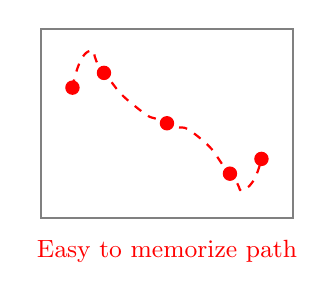
\begin{tikzpicture}[scale=0.8]
                % Box
                \draw[thick, gray] (0,0) rectangle (4,3);
                % 5 Points - positioned at extremes to look unrepresentative when sparse
                \filldraw[red] (0.5, {1.5 + 0.8*sin(0.5*90)}) circle (3pt);
                \filldraw[red] (1.0, {1.5 + 0.8*sin(1.0*90)}) circle (3pt);  % near peak
                \filldraw[red] (2.0, {1.5 + 0.8*sin(2.0*90)}) circle (3pt);
                \filldraw[red] (3.0, {1.5 + 0.8*sin(3.0*90)}) circle (3pt);  % near trough
                \filldraw[red] (3.5, {1.5 + 0.8*sin(3.5*90)}) circle (3pt);
                
                % Dashed line showing "Memorization" - overly wiggly overfitting
                \draw[red, dashed, thick] plot[smooth, tension=1.2] coordinates {
                    (0.5, {1.5 + 0.8*sin(0.5*90)}) 
                    (0.75, {1.5 + 0.8*sin(0.75*90) + 0.4})
                    (1.0, {1.5 + 0.8*sin(1.0*90)}) 
                    (1.5, {1.5 + 0.8*sin(1.5*90) - 0.3})
                    (2.0, {1.5 + 0.8*sin(2.0*90)}) 
                    (2.5, {1.5 + 0.8*sin(2.5*90) + 0.35})
                    (3.0, {1.5 + 0.8*sin(3.0*90)}) 
                    (3.25, {1.5 + 0.8*sin(3.25*90) - 0.3})
                    (3.5, {1.5 + 0.8*sin(3.5*90)})
                };
                
                \node[below, red, font=\small] at (2,-0.2) {Easy to memorize path};
            \end{tikzpicture}
        \end{column}
        
        % --- Large Data ---
        \begin{column}{0.50\textwidth}
            \centering
            \textbf{2. Large Data (Dense)}
            \vspace{0.5em}
            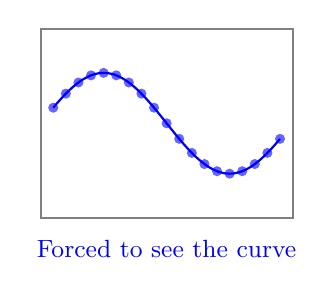
\begin{tikzpicture}[scale=0.8]
                % Box
                \draw[thick, gray] (0,0) rectangle (4,3);
                % Many points following a sine pattern
                \foreach \x in {0.2,0.4,0.6,0.8,1.0,1.2,1.4,1.6,1.8,2.0,2.2,2.4,2.6,2.8,3.0,3.2,3.4,3.6,3.8} {
                    \filldraw[blue!60] (\x, {1.5 + 0.8*sin(\x*90)}) circle (2pt);
                }
                
                % Smooth sine curve
                \draw[blue, thick, smooth] plot[domain=0.2:3.8, samples=50] (\x, {1.5 + 0.8*sin(\x*90)});
                
                \node[below, blue, font=\small] at (2,-0.2) {Forced to see the curve};
            \end{tikzpicture}
        \end{column}
    \end{columns}
    
    \begin{tcolorbox}[colback=green!5, colframe=green!40]
        \centering
        With more data, the "wiggly" memorization path becomes impossible. The model \textbf{must} learn the true underlying curve (Signal).
    \end{tcolorbox}
\end{frame}


% --- SLIDE 1: THE PROBLEM (VISUALIZATION) ---
\begin{frame}{Reduce Features}

    \begin{alertblock}{The Curse of Dimensionality}
        As you add more features (dimensions), the space grows exponentially. Your data becomes sparse, creating empty regions with no nearby data --- so the model is forced to \textbf{extrapolate where it has no support and overfits instead of generalizing}.
    \end{alertblock}
\end{frame}

% --- SLIDE 1: THE PROBLEM (VISUALIZATION) ---
\begin{frame}{The Curse of Dimensionality}

    \centering
    \textit{Visualizing the problem: Same 10 samples, increasing dimensions.}
    \vspace{0.5em}

    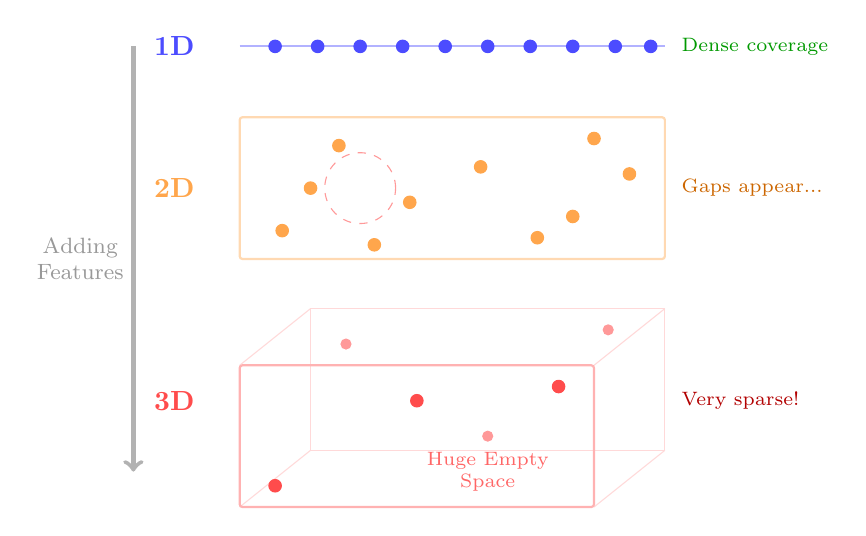
\begin{tikzpicture}[scale=0.9] 
        % --- 1D Line ---
        \node[left, font=\bfseries, blue!70] at (-0.5, 3) {1D};
        \draw[thick, blue!30] (0,3) -- (6,3);
        % 10 points
        \foreach \x in {0.5, 1.1, 1.7, 2.3, 2.9, 3.5, 4.1, 4.7, 5.3, 5.8} 
            \filldraw[blue!70] (\x, 3) circle (2.5pt);
        \node[right, font=\scriptsize, green!60!black] at (6.1, 3) {Dense coverage \checkmark};
        
        % --- 2D Square ---
        \node[left, font=\bfseries, orange!70] at (-0.5, 1) {2D};
        \draw[thick, orange!30, rounded corners=1pt] (0,0) rectangle (6,2);
        % 10 points scattered
        \filldraw[orange!70] (0.6, 0.4) circle (2.5pt);
        \filldraw[orange!70] (1.4, 1.6) circle (2.5pt);
        \filldraw[orange!70] (2.4, 0.8) circle (2.5pt);
        \filldraw[orange!70] (3.4, 1.3) circle (2.5pt);
        \filldraw[orange!70] (4.2, 0.3) circle (2.5pt);
        \filldraw[orange!70] (5.0, 1.7) circle (2.5pt);
        \filldraw[orange!70] (1.0, 1.0) circle (2.5pt);
        \filldraw[orange!70] (4.7, 0.6) circle (2.5pt);
        \filldraw[orange!70] (5.5, 1.2) circle (2.5pt);
        \filldraw[orange!70] (1.9, 0.2) circle (2.5pt);
        
        % Show empty regions
        \draw[red!40, dashed] (1.7, 1.0) circle (0.5cm);
        \node[right, font=\scriptsize, orange!80!black] at (6.1, 1) {Gaps appear...};
        
        % --- 3D Cube (FIXED PERSPECTIVE) ---
        \node[left, font=\bfseries, red!70] at (-0.5, -2) {3D};
        
        % 1. Define Coordinates
        % Front Face: (0, -3.5) to (5, -1.5)
        % Back Face: Shifted by (1, 0.8) -> (1, -2.7) to (6, -0.7)
        
        % 2. Draw Back Face (Behind)
        \draw[red!15, thin] (1,-2.7) rectangle (6,-0.7);
        
        % 3. Draw Connecting Lines (Corners to Corners)
        \draw[red!15, thin] (0,-1.5) -- (1,-0.7); % Top-Left
        \draw[red!15, thin] (5,-1.5) -- (6,-0.7); % Top-Right
        \draw[red!15, thin] (0,-3.5) -- (1,-2.7); % Bottom-Left
        \draw[red!15, thin] (5,-3.5) -- (6,-2.7); % Bottom-Right
        
        % 4. Draw Front Face (In Front)
        \draw[thick, red!30, rounded corners=1pt] (0,-3.5) rectangle (5,-1.5);
        
        % 5. Points (Scattered in "Depth")
        \filldraw[red!70] (0.5, -3.2) circle (2.5pt); % Front-ish
        \filldraw[red!70] (4.5, -1.8) circle (2.5pt); % Front-ish
        \filldraw[red!40] (1.5, -1.2) circle (2pt);   % Back-ish (lighter)
        \filldraw[red!40] (3.5, -2.5) circle (2pt);   % Middle
        \filldraw[red!40] (5.2, -1.0) circle (2pt);   % Far Back-Right
        \filldraw[red!70] (2.5, -2.0) circle (2.5pt); % Middle
        
        % 6. Labels
        \node[red!60, font=\scriptsize, align=center] at (3.5, -3.0) {Huge Empty\\Space};
        \node[right, font=\scriptsize, red!70!black] at (6.1, -2) {Very sparse!};
        
        % Vertical Arrow
        \draw[->, ultra thick, gray!60] (-1.5, 3) -- (-1.5, -3);
        \node[left, align=center, font=\footnotesize, gray!80] at (-1.5, 0) {Adding\\Features};
        
    \end{tikzpicture}
\end{frame}


% --- SLIDE 2: THE SOLUTION ---
\begin{frame}{The Curse of Dimensionality}

    \begin{block}{What Happens in High Dimensions?}
        \begin{itemize}
            \item[\textcolor{blue!70}{$\rightarrow$}] \textbf{1D:} 10 points densely cover the line.
            \item[\textcolor{orange!70}{$\rightarrow$}] \textbf{2D:} Same 10 points spread thin $\rightarrow$ gaps appear.
            \item[\textcolor{red!70}{$\rightarrow$}] \textbf{3D:} Mostly empty space $\rightarrow$ the model starts to find fake patterns in the noise just to bridge the gaps.
        \end{itemize}
    \end{block}

\end{frame}

\begin{frame}{The Solution: Feature Selection}

    \begin{block}{What Happens in High Dimensions?}
        \begin{itemize}
            \item[\textcolor{blue!70}{$\rightarrow$}] \textbf{1D:} 10 points densely cover the line.
            \item[\textcolor{orange!70}{$\rightarrow$}] \textbf{2D:} Same 10 points spread thin $\rightarrow$ gaps appear.
            \item[\textcolor{red!70}{$\rightarrow$}] \textbf{3D:} Mostly empty space $\rightarrow$ the model starts to find fake patterns in the noise just to bridge the gaps.
        \end{itemize}
    \end{block}

    \vspace{2em}
    
    \begin{tcolorbox}[colback=green!5, colframe=green!50, arc=3pt, boxrule=1pt]
        \centering
        \large \textbf{The Fix: Feature Selection}
        \vspace{0.5em}
        \normalsize
        \begin{itemize}
            \item Remove irrelevant features (noise) and keep only meaningful signals.
            \item This should push the data back down to lower dimensions where density is high.
        \end{itemize}
    \end{tcolorbox}

\end{frame}


% --- SLIDE 3: SUMMARY CHEAT SHEET ---
\begin{frame}{Summary: Diagnosing \& Fixing}

    \centering
    \renewcommand{\arraystretch}{1.5}
    \begin{table}[]
        \begin{tabular}{l|l|l}
            \hline
            \textbf{Problem} & \textbf{Diagnosis (Loss)} & \textbf{Mitigation (Fix)} \\ \hline
            \textbf{Underfitting} & \textcolor{blue}{Train High}, \textcolor{red}{Val High} & \begin{tabular}[c]{@{}l@{}} $\uparrow$ Increase Complexity \\ $\uparrow$ Add Features \end{tabular} \\ \hline
            \textbf{Overfitting} & \textcolor{blue}{Train Low}, \textcolor{red}{Val High} & \begin{tabular}[c]{@{}l@{}} $\downarrow$ Reduce Complexity \\ $\downarrow$ Remove Noise/Features \\ $\uparrow$ More Data \\ $\rightarrow$ Regularization (Next Days) \end{tabular} \\ \hline
            \textbf{Good Fit} & \textcolor{blue}{Train Low}, \textcolor{red}{Val Low} & \begin{tabular}[c]{@{}l@{}} $\checkmark$ All good! \end{tabular} \\ \hline
        \end{tabular}
    \end{table}

\end{frame}


% --- PART 4: DATA PREPARATION ---
\section{Data Preparation}

% --- SLIDE 1: TRANSITION ---
